% This is samplepaper.tex, a sample chapter demonstrating the
% LLNCS macro package for Springer Computer Science proceedings;
% Version 2.21 of 2022/01/12
%
\documentclass[runningheads]{llncs}
%
\usepackage[T1]{fontenc}
% T1 fonts will be used to generate the final print and online PDFs,
% so please use T1 fonts in your manuscript whenever possible.
% Other font encondings may result in incorrect characters.
%
\usepackage{graphicx}
% Used for displaying a sample figure. If possible, figure files should
% be included in EPS format.
%
% If you use the hyperref package, please uncomment the following two lines
% to display URLs in blue roman font according to Springer's eBook style:
%\usepackage{color}
%\renewcommand\UrlFont{\color{blue}\rmfamily}
%
\usepackage{xcolor}
\usepackage{amsfonts}
\usepackage{mathtools}
\usepackage{hyperref}
\usepackage{marginnote}
\usepackage{verbatim}
\usepackage{listings}
\usepackage{amsmath,mathrsfs,amssymb}
\usepackage{multirow}
\usepackage{wrapfig}
\usepackage{caption}
\usepackage{subcaption}
\usepackage{mathtools}
\usepackage{lmodern}

\newcommand{\term}[1]{\mbox{\texttt{\textbf{#1}}}}
\newcommand{\run}[2]{\term{run}^{#1}\,\left[#2\right]}
\newcommand{\todo}[1]{{\bf\color{red}#1}}
\newcommand{\rel}[3]{{#1}\xrightarrow{#2}{#3}}
\newcommand{\prg}[1]{\mbox{\lstinline|#1|}}
\newcommand{\precprec}{\prec\mathrel{\mkern-5mu}\prec}

\newcommand{\grc}[2]{{#1}\,\left<{#2}\right>}
\newcommand{\java}[1]{\texttt{#1}}
\newcommand{\primi}[1]{\mathbf{#1}}
\newcommand{\cc}[1]{\lfloor{#1}\rfloor}
\sloppy

\lstdefinelanguage{ocanren}{
keywords={run, conde, fresh, let, in, match, with, when, class, type,
object, method, of, rec, repeat, until, while, not, do, done, as, val, inherit,
new, module, sig, deriving, datatype, struct, if, then, else, open, private, virtual, include, success, failure, switch,
true, false, ocanren},
sensitive=true,
commentstyle=\small\itshape\ttfamily,
keywordstyle=\ttfamily\textbf,
identifierstyle=\ttfamily,
basewidth={0.5em,0.5em},
columns=fixed,
mathescape=true,
fontadjust=true,
literate={fun}{{$\lambda$}}1 {->}{{$\to$}}3 {===}{{$\equiv$}}1 {=/=}{{$\not\equiv$}}1 {|>}{{$\triangleright$}}3 {\\/}{{$\vee$}}2 {/\\}{{$\wedge$}}2 {^}{{$\uparrow$}}1
%{[]}{{\texttt|[]|}}1
,
morecomment=[s]{(*}{*)}
}

\lstdefinelanguage{ocaml}{
keywords={type, struct},
sensitive=true,
commentstyle=\small\itshape\ttfamily,
keywordstyle=\ttfamily\textbf,
%keywordstyle=\ttfamily\underbar,
identifierstyle=\ttfamily,
basewidth={0.5em,0.5em},
columns=fixed,
fontadjust=true,
literate={->}{{$\to$}}3 {=>}{{$\Rightarrow$}}3,
morecomment=[s]{(*}{*)}
}

\setlength{\belowcaptionskip}{-22pt}

\usepackage[nodisplayskipstretch]{setspace}

%\setlength{\abovedisplayskip}{-5pt}
%\setlength{\belowdisplayskip}{-5pt}

\renewcommand{\arraystretch}{0.3}

\pagestyle{plain}
%\usepackage{lineno}
%\linenumbers

\begin{document}
%
\title{Relational Solver for \textsc{Java} Generics Type System}
%
%\titlerunning{Abbreviated paper title}
% If the paper title is too long for the running head, you can set
% an abbreviated paper title here
%
\author{
  Peter Lozov\inst{1}\orcidID{0000-0003-3563-2828} \and
  Dmitry Kosarev\inst{1}\orcidID{0000-0002-6773-5322} \and
  Dmitry Ivanov\inst{2}\and
  Dmitry Boulytchev\inst{1}\orcidID{0000-0001-8363-7143}
}
%
\authorrunning{Dmitry Kosarev et al.}
% First names are abbreviated in the running head.
% If there are more than two authors, 'et al.' is used.
%
\institute{
Saint-Petersburg State University,\\
Universitetskaya emb., 7-9, 199034, St.Petersburg, Russia\\
\email{lozov.peter@gmail.com},\email{kakadu.hafanana@gmail.com},\email{dboulytchev@math.spbu.ru}\\
Saint-Petersburg,\\
\email{korifey@gmail.com}\\}
%
\maketitle              % typeset the header of the contribution
%
\begin{abstract}
  We present a solver for Java generics type system implemented using relational verifier-to-solver
  approach. The solver finds solutions for a system of subtyping inequations with free variables
  and thus can be used to determine a concrete type satisfying a set of constraints. The
  context of this work is symbolic execution for testing and verification of \textsc{Java} programs.
\keywords{\textsc{Java} generics \and relational programming \and relational solvers.}
\end{abstract}
%
%
%
% !TEX TS-program = pdflatex
% !TeX spellcheck = en_US
% !TEX root = main.tex


\section{Introduction}
\label{sec:intro}


One of distinguishable features of \miniKanren{} is the fact that it is a family of languages:
many languages may host different \miniKanren{} implementations.
For example, \faster{}\footnote{\url{https://github.com/michaelballantyne/faster-minikanren} (access date: \DTMdate{2024-06-06})} for \Scheme{} and \Racket{}, \CoreLogic{} for \textsc{Closure}, \OCanren{}~\cite{OCanren} for \OCaml{}, \Klogic{}~\cite{Klogic2023} for \Kotlin{} and others.
The users of these DSLs may want to compare expressive power of various flavor of miniKanren, specifics due to host language, and performance implications of choosing a different host language.


The straightforward solution is to rewrite a number of significant benchmarks for many implementation, as it done for other languages\footnote{\url{https://benchmarksgame-team.pages.debian.net/benchmarksgame/index.html} (access date: \DTMdate{2024-06-06})}.
Doing it manually is time consuming and error prone.
Due to low-level nature of relational programs, it is easy to make spelling mistakes, for example accidentally write wrong identifier in unification arguments.
(We did many of mistakes of this kind while porting programs from \OCanren{} to \Klogic{}.) Moreover, \miniKanren{} doesn't pardon relational programs that solve the same task: it was reported, that the order of conjuncts significantly affects~\cite{scheduling2022} performance even if the search does the same unifications.

The differences between host languages also complicate porting relational code.
For example, \Kotlin{} doesn't support currying and partial applications comparatively to \OCaml{}, and sometimes full $\eta$-expansion is needed.
Also, porting from dynamically typed languages like \Scheme{} to statically typed ones like \OCaml{} could be uneasy for newcomers to statically typed languages.
This porting could be not straightforward:
basic data representations in \OCaml{}/\Klogic{} (algebraic data types and classes with subclasses~--- sum types) is different from \Scheme{} (lists, i.e. arbitrary length tuples~--- product types).
This fact in some cases requires special constraints~\cite{Wildcards2023} to level the expressivity, and in other cases (like relational interpreters) allows to get rid of \emph{absento/symbolo} constraints.

Things could get even more complicated where we want to port larger projects which are using functional/relational approach where relational parts are intermixed with straightforward programming.
The developer is obliged to know relational approach, the original host general purpose language and to have experience  with a new host language.

In this paper we describe current status of our converter from relational \OCanren{} to \Klogic{} and \miniKanren{} in \Scheme{}.
At the moment only relational subset of \OCanren{} is supported, we don't support whole \OCaml{} language.
In next section we describe technical aspects of our approach and currently supported features.
In section \ref{sec:interpreter} we discuss transformation in relational interpreter~\cite{Untagged} from \OCanren{} to \Scheme{} and peculiarities of autogenerated implementation.



% !TEX TS-program = pdflatex
% !TeX spellcheck = en_US
% !TEX root = main.tex

\section{Relational Programming, Verifiers, and Solvers}
\label{sec:rel}

The implementation of our layout synthesizer employs the techniques of relational programming. Here
we briefly recollect what relational programming is and how the approaches and tools we use work.

Relational programming~\cite{TRS} is an approach based on the idea of describing programs as
relations. It can be considered as a branch of logic programming in which the use of
all non-relational constructs (side-effects, extra-logic features) is discouraged. In a
narrow sense relational programming amounts to writing programs in \textsc{miniKanren}~--- a
specifically designed for this purpose embedded DSL. Initially developed for \textsc{Scheme}/\textsc{Racket}
\textsc{miniKanren} later was ported for dozens of host
languages\footnote{\url{http://minikanren.org/\#implementations}}.
We, specifically, use a strongly typed \textsc{miniKanren} implementation for \textsc{OCaml}~\cite{ocaml}, called \textsc{OCanren}~\cite{OCanren}.
\textsc{miniKanren} uses the same theory of Horn clauses as \textsc{Prolog} but with a different
concrete syntax with explicit unification, conjunction, disjunction and fresh variable introduction, and
employs a different \emph{interleaving} search strategy~\cite{interleaving}, which is known to be complete~\cite{certified}.
Besides unification with occurs-check, enabled by default, \textsc{miniKanren} can be equipped with other
basic constraints like disequality constraint~\cite{disuni}, finite-domain constraints~\cite{cKanren}, or
constructs of nominal logic~\cite{aKanren}.

In the context of our work the most valuable property of \textsc{miniKanren} is its capability of expressing \emph{reverse computations}.
It is well-known~\cite{SemanticsModifiers,SemanticsModifiers1} that some complicated programs can be constructed as
the results of inversion of some other, much simpler, programs. In particular, a \emph{solver} for a
certain search problem can be considered as an inversion of its \emph{verifier}; it is rather a matter of common knowledge that verifying a
solution is, as a rule, much easier than finding one. The relational nature of \textsc{miniKanren} makes
inverse computations particularly easy~\cite{searchproblems}, which opens a way for program
synthesis~\cite{Untagged,WBirdSeven,PatternMatching}.

Another component of our approach is \emph{relational conversion}. In many cases (but not always!) it is easier to obtain a relational specification
from functional program than writing the one by hands. We use a tool, called \textsc{noCanren}, which converts programs written is a reasonable
subset of \textsc{OCaml} into correct-by-construction\cite{conversion} \textsc{OCanren} specifications.

We demonstrate the roadmap of our approach by the following observable example. Let us have a program
shown in Fig.~\ref{fun_vs_rel}\subref{funadd} which adds two natural numbers in Peano form. Its relational counterpart,
acquired via relational conversion (not literally, but in equivalent form), is shown in Fig.~\ref{fun_vs_rel}\subref{reladd}.
Comparing both of them we can notice that pattern-matching was replaced by disjunction (\lstinline[language=ocanren,basicstyle=\small]|\/|)
and unification (\lstinline[language=ocanren,basicstyle=\small]|===|), data-flow dependent computations with conjunction (\lstinline[language=ocanren,basicstyle=\small]|/\|),
and fresh variables can be allocated when needed; the postfix ``$^o$'' is traditionally used to distinguish relational definitions. Unlike its functional
counterpart the relational specification has \emph{three} arguments \lstinline[language=ocanren,basicstyle=\small]|x|, \lstinline[language=ocanren,basicstyle=\small]|y|,
and \lstinline[language=ocanren,basicstyle=\small]|z|, each of which can contain fresh (initially undefined) variables.
The evaluation of construction \lstinline[language=ocanren,basicstyle=\small]|run$^*$ {add$^o$ x y z}| returns all substitutions for these
fresh variables which make the relation $\{(\mbox{\texttt x}, \mbox{\texttt y}, \mbox{\texttt z})\in\mathbb{N}^3\, |\, \mbox{\texttt x+y=z}\}$ hold, represented as a \emph{lazy stream of answers}. This stream can
then be inspected in a host functional application to retrieve individual answers. Thus the same specification can be equally used for plain addition,
subtraction or decomposition of a number into two summands.

\begin{figure}[t]
  \begin{subfigure}[t]{0.5\textwidth}
  \begin{lstlisting}[language=ocanren,basicstyle=\small]
   let rec add x y =
     match x with
     | O    -> y
     | S x' -> S (add x' y)
  \end{lstlisting}
  %\vskip12mm
  \caption{Functional addition}
  \label{funadd}
  \end{subfigure}
  \begin{subfigure}[t]{0.5\textwidth}
    \begin{lstlisting}[language=ocanren,basicstyle=\small]
  let rec add$^o$ x y z = ocanren {
    x === O /\ z === y \/
    fresh x', z' in
      x === S x' /\
      z === S z' /\
      add$^o$ x' y z'
  }
    \end{lstlisting}
    \caption{Relational addition}
    \label{reladd}
  \end{subfigure}
  \caption{Functional vs. relational addition of Peano numbers}
  \label{fun_vs_rel}
\end{figure}

\section{Java Generics}

Here we briefly describe the relevant subpart of \textsc{Java} type system. All
information in this section is directly derived from the Java Language Specification~\cite{JLS}.
We also refrain from reiterating on the non-generic part of \textsc{Java} type system assuming the reader's familiarity
with the concepts of reference types, arrays, classes, interfaces, and inheritance.

The subsystem we are dealing with contains generic class/interface types $\grc{C}{\mathscr{T}^*}$, array types $\mathscr{T}\mbox{\java{[]}}$,
type variables $\alpha^\mathscr{T}_\mathscr{T_\bot}$, intersection types $\bigcap\,\mathscr{T}$ and  $\primi{null}$ type.
Here $\mathscr{T}$ denotes a type, $\mathscr{T}_\bot$~--- an optional type.
Type variables are bounded in the sense that they always have a certain \emph{upper bound}. This upper
bound can be either specified explicitly or assumed to be \java{java.lang.Object}. In addition
to the upper bound a type variable can be equipped with a \emph{lower bound}. The lower bound can only
be derived implicitly as a result of \emph{capture conversion} (see below). We denote the upper bound of a variable
by  superscript and lower~--- by subscript.

Generic class (or interface) is a class/interface which is equipped with a number of
type parameters. In generic class declaration these parameters can only be type
variables with specified upper bounds. Additionally a number of \emph{direct supertypes} (notation: ``$\prec$'')
can be specified for a generic class/interface:

\[
\grc{C}{\alpha_1^{U_1}\dots \alpha_k^{U_k}}\prec\grc{S_1}{T^1_1\dots T^1_{n_1}}\dots\grc{S_m}{T^m_1\dots T^m_{n_m}}
\]

Here $C$ is the class/interface being declared, $\alpha_i^{U_i}$~--- its generic parameters with upper
bounds, $S_i$~--- its direct supertypes, among which only one type can be a class type, $T^j_l$~--- type
parameters for direct supertypes, which may contain the occurrences of $\alpha_i$; note: neither of $T^j_l$ can be
an intersection type.

Type variables in scopes of their declarations behave like regular types; the scope of a type variable is
determined by the position of its introduction (either generic class/interface or generic method). It
is unclear what is the scope of type variables introduced implicitly as a result of capture
conversion, but this might be irrelevant to the problem we are dealing with.

Intersection types can not be declared explicitly; the only positions in which they can be specified are
upper bounds of type parameters in generic class/interface declarations. However intersection types can be derived
as a result of capture conversion.

Null type is an artificial transparent type with no explicit representation. It is assumed to be a subtype for
every other reference type.

Besides regular types generic classes can be applied to \emph{wildcard types}. A wildcard is an anonymous
type variable (notation: ``\java{?}'') equipped, as a regular type variable, with upper bound and optional lower bound
neither of which can be of intersection type. If no upper bound is specified explicitly then \java{java.lang.Object} is implicitly assumed.
It is important that wildcards can not be used to parameterize direct supertypes in generic class/interface declarations.
Array types can not be directly parameterized by wildcards.

To establish the subtyping relation (denotation: ``$\precprec$'') between types parameterized by wildcards two additional
notions are introduces.

The first one is \emph{contains} relation ``$\supseteq$'':

\[
\begin{array}{rclcl}
  \java{?}^T&\supseteq&\java{?}^S&,&T\precprec S \\[2mm]
  \java{?}^T&\supseteq&\java{?}&& \\[2mm]
  \java{?}_T&\supseteq&\java{?}_S&,&S\precprec T\\[2mm]
  \java{?}_T&\supseteq&\java{?}&& \\[2mm]
  \java{?}_T&\supseteq&\java{?}^\java{java.lang.Object}&& \\[2mm]
  T&\supseteq& T&&\\[2mm]
  T&\supseteq&\java{?}^T&&\\[2mm]
  T&\supseteq&\java{?}_T&&
\end{array}
\]

This relation in essence is a routine check that a collection of types designated by the ``right'' type is
contained in a collection of types designated by the ``left'' one.

The second is \emph{capture conversion}. Informally, capture conversion replaces a \emph{nameless} wildcard type
argument by a freshly introduced \emph{named} type variable, thus ``capturing'' some concrete (but statically unknown)
type in a certain context. The motivation for introducing capture conversion is as follows: let us have
some value of a wildcard-parameterized type, say, some collection of type $\grc{Collection}{?}$. Without capture
conversion we would be incapable of dealing with individual elements of this collection (since a wildcard is not a type,
but rather a way to to describe a certain parameterization). From a type-theoretic standpoint wildcards introduce a
certain form of \emph{existential} types with capture conversion serving as a limited form of opening construct~\cite{tapl}.
The detailed theory and the discussion of properties for the wildcard-related fragment of Java Generics type system
can be found in~\cite{wild}.

Capture conversion is defined as follows. Let $\grc{C}{T_1\dots T_k}$ be a generic class/interface type where some of $T_i$ are wildcards. Let
$\beta_i^{U_i}$ be the $i$-th type parameter of $C$'s declaration. Then capture conversion of
$\grc{C}{T_1\dots T_K}$ is the type $\grc{C}{\cc{T_1}\dots \cc{T_k}}$ where the transformation
``$\cc{\bullet}$'' is defined as follows:

\[
\cc{T_i}=\left\{
\begin{array}{lll}  
  \alpha^{U_i[\beta_j\gets \cc{T_j}]}_\primi{null}      &\mbox{if }        T_i=\java{?}  &\mbox{($\alpha$ is a fresh type variable)}\\[5mm]
  \alpha^{B\cap U_i[\beta_j\gets \cc{T_j}]}_\primi{null} &\mbox{if }        T_i=\java{?}^B &\mbox{($\alpha$ is a fresh type variable)}\\[5mm]
  \alpha^{U_i[\beta_j\gets \cc{T_j}]}_B               &\mbox{if }        T_i=\java{?}_B &\mbox{($\alpha$ is a fresh type variable)}\\[5mm]
  T_i                                           &\mbox{otherwise}  & 
\end{array}\right.
\]

Here ``$[\bullet\gets\bullet]$'' denotes a (simultaneous) substitution of type variables with some types. Note, in capture conversion
type parameters of the class under conversion are substituted with the results of the conversion in all bounds.

The subtyping relation ``$\precprec$'', which is the principle notion for the problem we are dealing with, is defined as a reflexive-transitive
closure of the direct supertype relation ``$\prec$''. We already described one case of direct supertyping, the others are as follows:

\[
\begin{array}{rclcl}
  I & \prec & \java{java.lang.Object} &,& \mbox{($I$ is an interface with no}\\
    &       &                         & &\mbox{direct superinterface)}\\[2mm]
  \grc{C}{T_1\dots T_k} & \prec & \grc{C}{S_1\dots S_k} &,& \forall i\, .\, S_i\supseteq T_i\\[2mm]
  \grc{C}{T_1\dots T_k} & \prec & S &,& \grc{C}{\cc{T_1}\dots \cc{T_k}}\prec S\\[2mm]
  \bigcap T_i & \prec & T_i && \\[2mm]
  \alpha^{\bigcap T_i} & \prec & T_i &&\\[2mm]
  T & \prec & \alpha_T && \\[2mm]
  \primi{null} & \prec & T &&\\[2mm]
  T\java{[]} & \prec & S\java{[]} &,& T\prec S\\[2mm]
  \java{java.lang.Object[]} & \prec & \java{java.lang.Object} &&  \\[2mm]
  \java{java.lang.Object[]} & \prec & \java{java.lang.Cloneabe} && \\[2mm]
  \java{java.lang.Object[]} & \prec & \java{java.io.Serializable} &&
\end{array}
\]

Note: the notions ``$\supseteq$'', ``$\prec$'', and ``$\precprec$'' are defined mutually recursive: ``$\precprec$'' is used
to define ``$\supseteq$'', which is used to define ``$\prec$'', which, in turn, is the basic relation to define ``$\precprec$''.

\section{Relational Subtyping Solver}
\label{sec:solver}

The approach of verifier-to-solver conversion relies on the implementation of functional verifier for the problem in question. In our
case such verifier should test if two given ground types are in the subtyping relation. This, in particular, requires implementation
of capture conversion, ``contains'' relation, and direct subtyping verifier. Then a reflexive-transitive closure of the latter has to
be implemented. The functional verifier is then converted into relational form which by construction delivers a subtyping solver for
non-ground types with free variables.

A simple observation, however, makes its obvious that it is in fact much easier to implement reflexive-transitive closure directly
in relational language. Indeed, given relation $R$ its reflexive-transitive $R^*$ closure can be expressed by just

\[
R^*\,(x,\, y) = R\, (x,\, y)\vee x\equiv y\vee\exists\, z\,.\,R\,(x,\,z)\wedge R^*\,(z,\,y)\eqno{(\star)}
\]

which can be easily directly encoded in \textsc{OCanren}. However, from the implementation standpoint the application of this technique
imposes a certain problem since ``$\prec$'' and ``$\precprec$'' are mutually recursive, and we expect ``$\prec$'' to be obtained as a
result of relational conversion of functional implementation.

Functional verifier is implemented in \textsc{OCaml} in a straightforward manner: we encode types as data structures of certain types and give a
direct implementation for all components of subtyping relation except the transitive closure. All these definitions are ``wrapped'' in a
functor (an \textsc{OCaml} module parameterized by a module) which takes \emph{class table} as a parameter. The class table
contains the definitions of relevant set of classes with their direct supertyping encoding, description of their type parameters, etc.
The concrete contents of the class table is supplied by the symbolic execution engine.

To build a mixture of relationally-converted code and relational implementation of transitive closure we use open recursion: the functional
implementation of direct supertyping relation ``$\prec$'' is parameterized by subtyping relation  ``$\precprec$''. In functional implementation
the knot is tied not by transitive closure of ``$\prec$'' but by ``$\prec$'' itself:

\begin{lstlisting}[language=ocanren,mathescape=true]
  let rec ($\precprec$) ta tb = ta $\prec$ tb 
  and ($\prec$) ta tb     = Verify.($\prec$) ($\precprec$) ta tb
\end{lstlisting}

Here ``\lstinline|Verify|'' is a module acquired by an instantiation of the verifier for a simple hand-written testing class table.
Thus, functional verifier can only check the subtyping of types no more then two ``steps'' away from each other.

The next step is applying relational conversion for this functional verifier. For technical reasons this requires a mild
``massaging'' of initial \textsc{OCaml} implementation: arrays (more efficient in functional world) have to be replaced
with lists, and some changes have to be made in order to compensate for the incompleteness of current relational
conversion implementation.
After the relational conversion and the parameterization of verifier functor with a class table a proper recursive knot is tied by a transitive closure of ``$\prec$'', which
completes the construction of the solver. While functional verifier can only work for ground types and return a boolean value, its relational counterpart
searches for all substitution for free variables in incomplete types is order to make them subtype each other.

Our first evaluation discovered the fact that the solver was unsound~--- it established the subtyping relation for two arbitrary types. This finding constitutes a drastic
contradiction with the theory which predicts that the solver has to be correct by construction. The careful analysis, however, discovered that functional
verifier was unsound as well! The reason was very simple: let us have two arbitrary types $A$ and $B$. To establish, for example, that $A \precprec B$, take a
type variable $\alpha^B_A$ with upper bound $B$ and lower bound $A$. Then, by definition

\[
A\precprec \alpha^B_A \wedge \alpha^B_A\precprec B \Rightarrow A\precprec B
\]

In the JLS there were no explicit requirement for lower/upper bounds of type variables to respect the subtyping relation, thus this requirement was not
encoded in the verifier. Another finding of the evaluation was that, contrary to the expectation, the direct supertyping relation is actually
reflexive (in full accordance with the JLS).

After fixing the unsoundness we found that the performance of the solver was very low: it took seconds to come up with the first solution even for
small hard-written class tables. After a careful analysis we come up with the following optimizations.

First, we changed the representation of class/interface identifiers. In functional verifier all identifiers were represented by integer numbers which,
under relational conversion, were tuned into natural numbers in Peano form (essentially, lists). At the same time as no transformation are
performed on identifiers (besides equality checks) this representation is excessive. We manually reverted the identifiers representation to
integers.

Then, we optimized the search in class tables. Functional verifier sometimes needs to find a declaration of a class/interface by identifier, or
find a superclass/superinterface for a class given this class identifier, etc. Under relational conversion all these procedures
take form of disjunctions of the length proportional to the size of the class table. However, when some of the involved identifiers
are ground the search can be optimized: we can query a precompiled optimized map-like structure of the class table to filter out
only relevant information and synthesize the residual disjunction at the runtime. We call this optimization \emph{dynamic class table specialization}.

Finally, we optimize the evaluation of transitive closure based on the groundness analysis of the arguments. For example, if we need to find a certain
$x$ such that $R^*\,(x,\,y)$ where $y$ is \emph{ground}, then the following (equivalent to $(\star)$) procedure of finding transitive closure is
found to be more efficient:

\[
R^*\,(x,\, y) = R\, (x,\, y)\vee x\equiv y\vee\exists\, z\,.\,R\,(z,\,y)\wedge R^*\,(x,\,z)
\]

So, in our implementation the groundness analysis (performed on the fly) chooses one of a few versions of transitive closure calculations.
We call this optimization \emph{dynamic transitive closure evaluation}.

With all of these optimizations enabled our solver finally can demonstrate a reasonable performance. We present the results of the evaluation
in the next section\footnote{Source code is available online: \url{https://github.com/Lozov-Petr/JGS/tree/LOPSTR-2023}}. 

\section{Evaluation}
\label{sec:eval}

We evaluated our solver for a class table containing more than 40000 classes exported by the symbolic execution engine using
nine benchmark queries of various shapes. By the specifics of using the solver as a part of symbolic execution engine we
switched off the capture conversion. The motivation is simple: the symbolic execution engine is interested only in
such types instances of which can be created at runtime. Thus, capture conversion can only be applied in a \emph{forward}
direction which eliminated wildcards. With capture conversion enabled in the relational solver it could also be
applied in reverse direction, introducing superfluous wildcards which could not be utilized properly.

The results are presented in Fig.~\ref{fig:eval-diagram} in the form of
a bar chart. Here the groups of four bars correspond to different benchmarks, each bar in the group corresponds to a one of
four versions of the solver (left-to-right): with no optimizations, with dynamic transitive closure evaluation only, with dynamic class table specialization only,
and with both optimizations enabled.

The benchmark queries are as follows:

\begin{enumerate}
   \item $\alpha$ $\precprec$ \java{java.util.List<Object>}
   \item $\alpha$ $\precprec$ \java{java.util.RandomAccess} $\land$ \\
          $\alpha$ $\precprec$ \java{java.util.AbstractCollection<Object>}
    \item $\alpha$ $\precprec$ \java{java.util.AbstractCollection<Object>} $\land$ \\
          $\alpha$ $\precprec$ \java{java.util.RandomAccess} 
    \item $\alpha$ $\precprec$ \java{java.util.AbstractCollection<Object>} $\land$ \\
          $\alpha$ $\precprec$ \java{java.util.RandomAccess} $\land$ \\
          $\alpha$ $\precprec$ \java{java.util.List<Object>}
    \item \java{javax.management.AttributeList} $\precprec$ $\alpha$
    \item \java{javax.management.AttributeList} $\precprec$ $\alpha$ $\land$ \\
          \java{kotlinx.collections.PersistentVector<Object>} $\precprec$ $\alpha$
    \item \java{kotlinx.collections.PersistentVector<Object>} $\precprec$ $\alpha$ $\land$ \\
          \java{javax.management.AttributeList} $\precprec$ $\alpha$ $\land$ \\
          \java{com.google.common.collect.ImmutableSortedSet<Object>} $\precprec$ $\alpha$
    \item \java{kotlinx.collections.PersistentVector<Object>} $\precprec$ $\alpha$ $\land$ \\
          $\alpha$ $\precprec$ \java{java.util.List<Object>}
    \item $\alpha$ $\precprec$ \java{java.util.List<Object>} $\land$ \\
          \java{kotlinx.collections.PersistentVector<Object>} $\precprec$ $\alpha$
\end{enumerate}


%\begin{itemize}
%    \item The first founr queries are systems of one, two, and three inequations with upper bounds only 1, 2 and 3 upper bounds for standard collection classes and interfaces \java{List}, \java{Abstract%Collection} and \java{RandomAccess}. Note, the 2nd and the 3rd queries are the same 2 upper bounds but with opposite order.
%    \item The next 3 queries are 1, 2 and 3 lower bound for concrete collection classes \java{AttributeList}, \java{PersistentVector} and \java{ImmutableSortedSet}.
%    \item The last 2 queries consist of one upper bound and one lower bound. These bounds the same for both queries but with opposite order.
%\end{itemize}

\begin{figure}[t]
  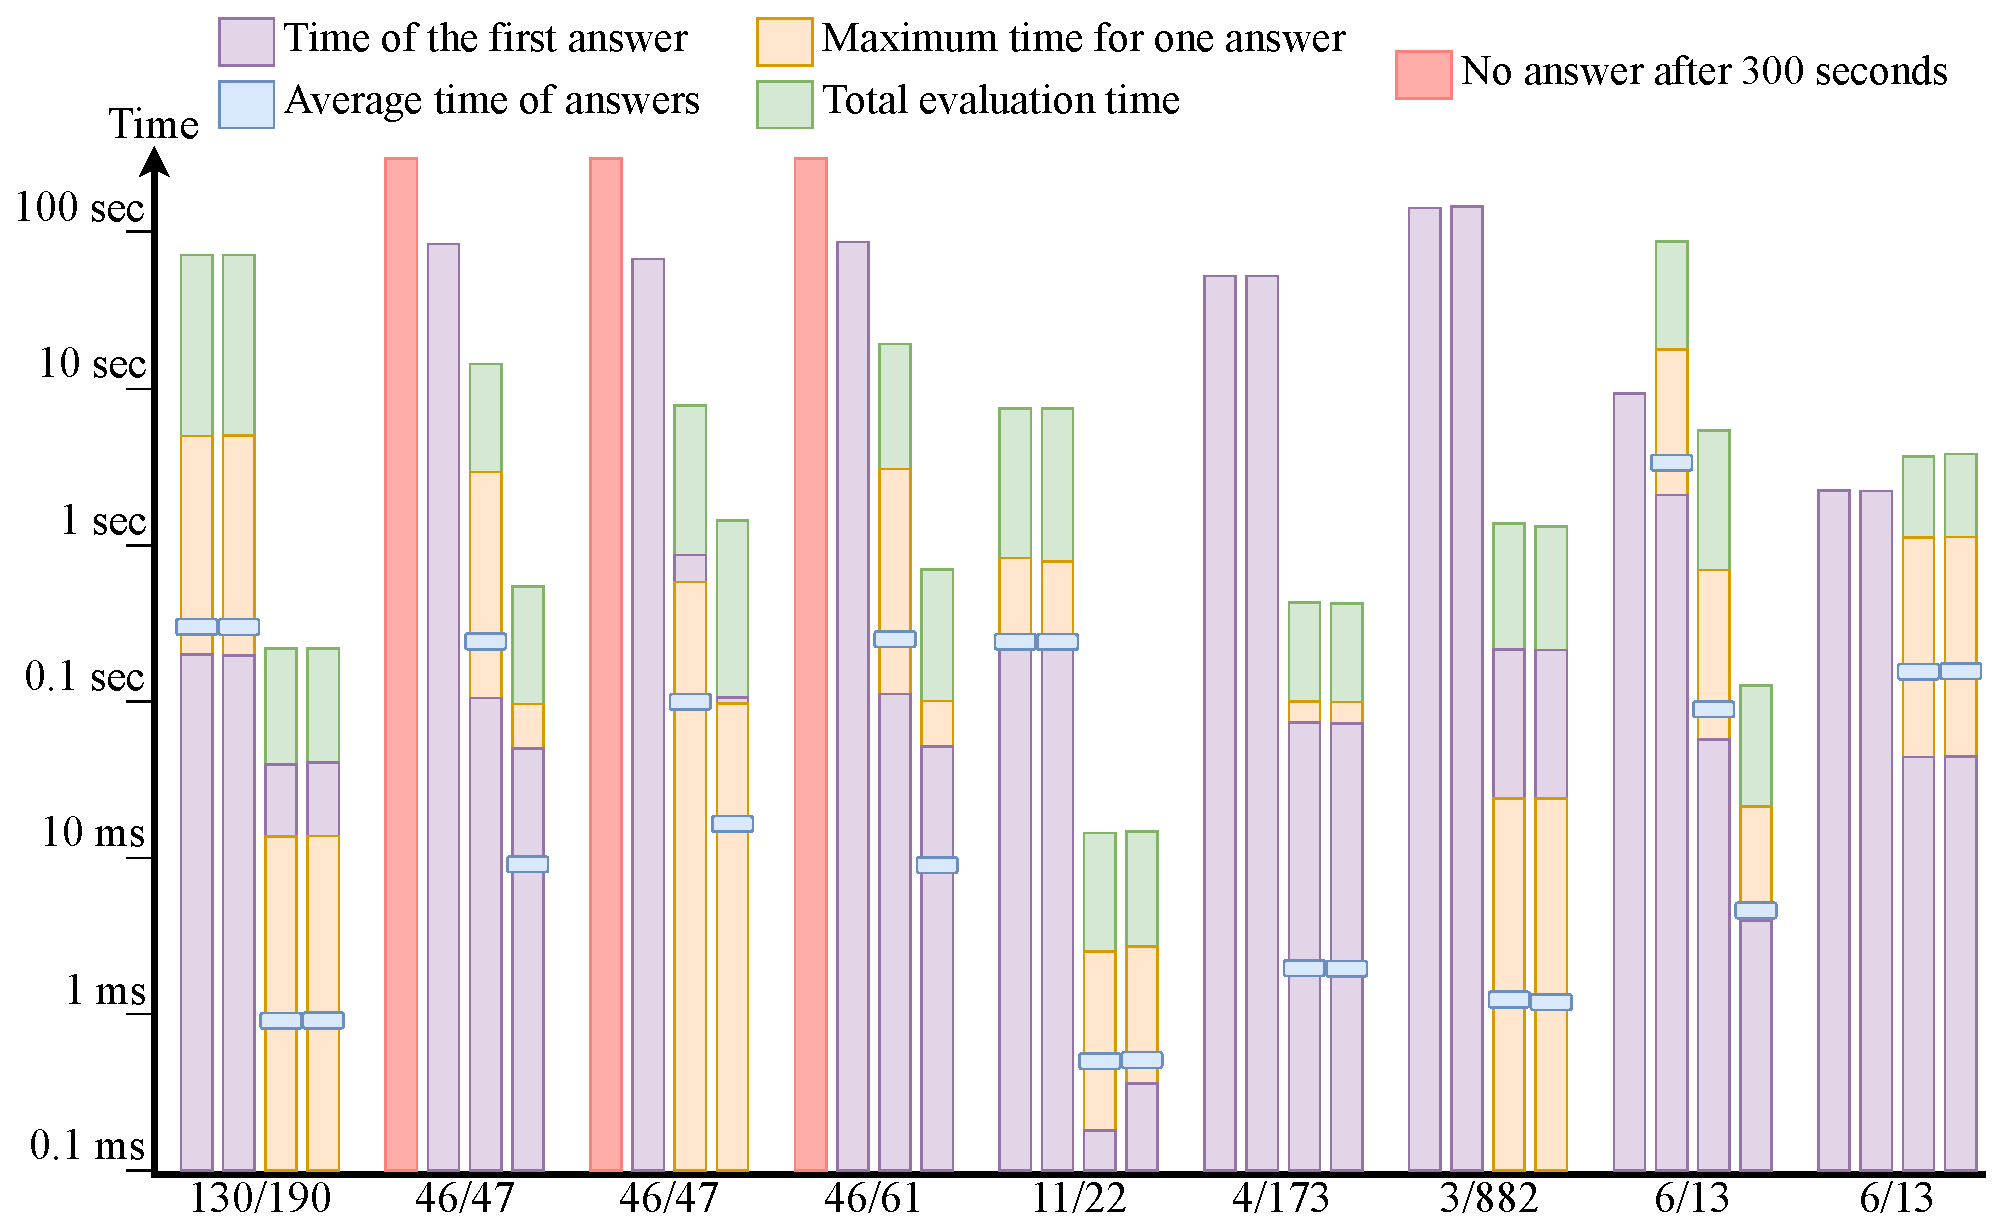
\includegraphics[width=1\textwidth]{eval_diagram.eps}
  \caption{Evaluation results}
  \label{fig:eval-diagram}
\end{figure}

 For each query we evaluated two quantitative measures: the overall number of answers (shown as a numerator
under corresponding benchmark) and the number of unique answers (shown as a denominator). Also we evaluated four time measures: the time of calculating the first answer (this time includes the time
spent on the pre-calculations required by dynamic table specialization), the maximal time for one answer (not including the first answer time), the average time taken over all answers,
and the total evaluation time. We also limited the evaluation time to 300 seconds; in a few cases we either received only a part of the answers (in this case, only the time for
calculating the first answer is indicated), or we did not receive a single answer (in this case, the red column is shown in the bar chart). All measurements are presented in a logarithmic
scale.

As we can see from the results, dynamic transitive closure in some cases improves the performance by an order of magnitude (if there is an upper bound among the
second and subsequent inequations), dynamic specialization of the table always improves the result by an order of magnitude, but the best performance is achieved when using both optimizations.
It is also noteworthy that the performance of the solver depends on the order of inequations in the query (the benchmarks 3 and 4, 8 and 9 differ only in this aspect). Also, it can be noted that
solving the inequations with lower bounds delivers a large number of duplicate answers.

We can conclude that the optimized version of the solver shows promising performance results, but the problems of performance dependance on the order of bounds and
the presence of duplicates require further research.


\section{Conclusion and future work}

We presented an approach for pattern matching implementation synthesis using relational programming. Currently, it demonstrates a good performance only
on a very small problems. The performance can be improved by searching for new ways to prune the search space and by speeding up the implementation of
relations and structural constraints. Also it could be interesting to integrate structural constraints more closely into \textsc{OCanren}'s core.
Discovering an optimal order of samples and reducing the complete set of samples is another direction for research.

The language of intermediate representation can be altered, too. It is interesting to add to an intermediate language so-called \emph{exit nodes}
described in~\cite{maranget2001}. The straightforward implementation of them might require nominal unification, but we are not aware of any
\textsc{miniKanren} implementation in which both disequality constraints and nominal unification~\cite{alphaKanren} coexist nicely.

At the moment we support only simple pattern matching without any extensions. It looks technically easy to extend our approach with
non-linear and disjunctive patterns. It will, however, increase the search space and might require more optimizations.






%
% ---- Bibliography ----
%
% BibTeX users should specify bibliography style 'splncs04'.
% References will then be sorted and formatted in the correct style.
%
\bibliographystyle{splncs04}
\bibliography{main}
%
\end{document}
